\chapter{Ergebnisse}
\label{chap:results}

% Dieses Kapitel enthält die gewonnenen Daten und ist deshalb in wissenschaftlicher Hinsicht besonders wichtig. Es dürfen nur Ergebnisse, die für die Fragestellung relevant sind, aufgeführt werden. Dazu können aber auch Negativergebnisse gehören. Die Fragen der Einleitung müssen mit den vorgestellten Ergebnissen zu beantworten sein.
% 
% Die Ergebnisse sollten mit Hilfe von Abbildungen und Tabellen möglichst übersichtlich dargestellt werden. Der Text sollte möglichst kurz gehalten werden und nicht die Informationen der Abbildungen und Tabellen wiederholen. Emotionen wie z.B. Erstaunen oder Entsetzen sollten vermieden werden. In den statistischen Auswertungen müssen neben Mittelwerten auch Streuungsmasse und Stichprobengrössen angegeben werden.
% 
% Es muss immer klar sein, ob es sich um eigene oder fremde Ergebnisse (z.B. aus Literaturrecherchen) handelt. Bei fremden Ergebnissen muss im Text auf die Herkunft verwiesen werden (siehe 2.8). Wörtliche Zitate sollten vermieden werden.

%  \begin{compactenum}[a)] % chktex 9 chktex 10 chktex 17
%      \item Auszug aus einer zoologischen Untersuchung zur Diversität von Arthropoden in voralpinen Flachmooren:
%          „In den untersuchten Gebieten konnten 63 Tagfalterarten aus 6 Familien nachgewiesen werden (Anhang IV). 16 Arten (25\%) gelten als typische Moorindikatoren und 23 Arten (37\%) erscheinen auf der Roten Liste der gefährdeten Tagfalter der Schweiz (Duelli 1994). Die Individuenzahl der Arthropoden nahm mit zunehmender Höhe ab (p < 0.05). Während in der tiefen Höhenstufe durchschnittlich 249 Tiere pro Gebiet gefangen wurden, waren es in der mittleren Höhenstufe 236 und in der höchsten nur noch 191 Individuen.“
%      \item Auszug aus einer sozialwissenschaftlichen Untersuchung über Engagement und Mobilität:
%          „Die Gesamtmobilität der Befragten liegt bei 12'600 km (Bezugsjahr 1994). Sie hat im erfragten Zeitraum um 12\% zugenommen (von 11'300 km auf 12'600 km). Der grösste Teil dieses Anstiegs geht auf die Ferienmobilität zurück, die im Schnitt von 6'400 km auf 7'300 km zugenommen hat. Die genannten Mobilitätswerte liegen deutlich unter dem Schweizer Durchschnitt.“
%  \end{compactenum} % chktex 17

\section{MATLAB-interne Methode \textit{activecontour}}
\label{sec:results:matlab}
Mittels der MATLAB-internen Methode wurde die Fraktur als zusammenhängende Region erkannt und könnte somit problemlos extrahiert werden. Die Erkennung dauert im Schnitt rund 4.3 Sekunden. Das Resultat ist in Abbildung~\ref{fig:matlab_result} ersichtlich.

\begin{figure}[h!]
    \centering
    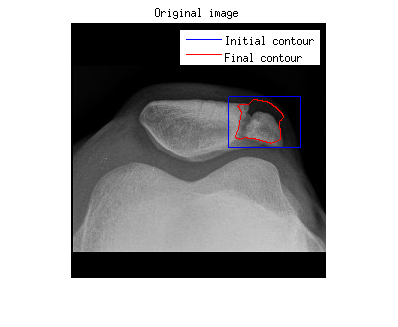
\includegraphics[scale=0.5]{images/matlab_result.png}
    \caption{Resultat der Erkennung der gewünschten Region mittels der MATLAB-internen Methode \textit{activecontour}\protect\footnotemark[1]{}}
\label{fig:matlab_result}
\end{figure}
\footnotetext[1]{Eigene Darstellung mittels MATLAB}

\section{Eigene Implementation}
\label{sec:results:own}
Auch mit dieser Methode wurde die Fraktur als zusammenhängende Region erkannt und könnte somit problemlos extrahiert werden. Die Erkennung dauert im Schnitt rund 3.5 Sekunden. Das Resultat ist in~\autoref{fig:ownimpl_result} abgebildet.

\begin{figure}[h!]
    \centering
    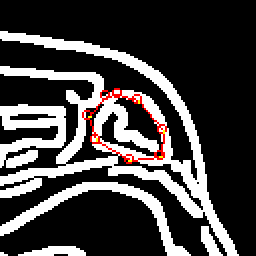
\includegraphics[scale=0.5]{images/ownimpl_result.png}
    \caption{Resultat der Erkennung der gewünschten Region anhand der eigenen Implementation in MATLAB\protect\footnotemark[1]{}}
\label{fig:ownimpl_result}
\end{figure}
